\chapter{Indirect Methods of Proof}

\begchap{T}hus far we have focused on ways to directly prove or disprove a statement. However, we can indirectly prove a statement via two other statements we discussed in Chapter 2. The first, and perhaps most important, is the negation. If the original statement is true, the inverse is false, and vice versa. Thus, if we know the negation is false, we know the original statement is true, and use this as a means of proof. This method is called proof by contradiction. The second important, albeit rare, type of proof is proof by contrapositive. Recall again that if a statement is true, then its contrapositive must be true, and vice versa. Thus, proof of the contrapositive proves the original statement itself. We will further analyze both techniques in this chapter.

\section{Contradiction}
To begin proof by contradiction, we will give an unusual example to start that will perhaps provide a little more motivation behind proof by contradiction. 

\begin{example}
Assume in the suburb of Canineville, Bob is accused of unlawfully eating his neighbor Alice's treats. You are Bob's lawyer, trying to prove his innocence. 
\end{example}
Now, proving innocence directly is difficult, since you cannot just go and assert that Bob did not steal - that would not prove anything. Thus, you search for a different type of logic.  
\begin{proof}
You begin your proof of Bob's innocence. You first begin by assuming the prosecution is correct, that Bob did unlawfully eat the treats. This would require Bob to be at Alice's house, since Alice's treats were in her house. Next, you know that the prosecution claimed the time of the theft was between 12:00 pm and 1:00 pm, and as you assume the prosecution is correct, you take this to be true as well. But then, you check the security camera footage, which shows Bob peacefully sleeping in his own house, from 11:30 am to 3:00 pm! You can see why this is a problem now. You conclude to the courtroom, with convincing evidence, that there is a contradiction: if Bob had stolen the treats, then Bob would need to be at Alice's house. However, Bob was at his house at the same time the treats were eaten! You conclude that Bob must be innocent since if Bob were to steal the treats, he would have to be in multiple places at the same time.
\end{proof}

Lawyers call this an alibi, though in mathematics, we call this proof by contradiction. We wish to prove some statement $I$. We know that both $I$ and $\neg I$ cannot be true at the same time. if $\neg I$ cannot be true, then $I$ itself must be true. (Very rarely, neither can be true but we tend to avoid such scenarios in mathematics, $I$ and $\neg I$ combines will usually cover the entire range of possibilities). We assume $\neg I$ to be true, then follow its logical consequences, leading to some sort of contradiction, or something impossible. In the above case, the impossibility was that Bob could not be in two places at the same time. However, keep in mind that the impossibility does not need to directly contradict $\neg I$, it could just be some minor logical inconsistency that arises if we assume $\neg I$ to be true. Such an inconsistency could be, that the footprints on the ground had 4 pawprints but Bob is a unique dog who walks standing up, leaving only 2 pawprints per step. It could be something else that is impossible, something that violates a known fact (e.g. if $\neg I$ meant $1=0$), or something that contradicts the initial conditions. You have seen the second type of proof by contradiction already. 

Consider the following system of equations.
\[
\begin{cases}
2x+y=5 \\
6x+3y=6
\end{cases}
\]
Now take the second equation, and we can factor out a 3 from both sides, effectively reducing the system of equations.
\[
\begin{cases}
2x+y=5 \\
2x+y=2
\end{cases}
\]
You can begin to see the problem...
To make it more clear and formal, we can subtract the second equation from the first (or first from second, order does not matter here), which gives
\[
0 = 3
\]
which is a clear contradiction of known facts. We have used this in early school to prove that the system of equations has no solution. More formally, if there did exist a solution $(x, y)$ to the system of equations, then we would have that $0 = 3$, which is a contradiction. Note that we could also derive this contradiction via substitution, since both left-hand sides of the equations are the same after simplification. However, the fact stands that since we get a logical contradiction, the statement that there exists a solution to this system of equations cannot be true. This time, our statement $I$ is that there does not exist a solution to the system of equations, where $\neg I$ is along the lines of "there exists $(x, y) \in \mathbb{R}^2$ such that the system of equations has a solution". 

One of the most famous proofs, one which you will inevitably see at some point during your career in mathematics, is the proof that $\sqrt{2}$ is an irrational number. We will use this example to demonstrate a more formal proof by contradiction, and one that is worth remembering for your journey in math!

\begin{example}
    Prove that $\sqrt{2}$ is an irrational number. 
\end{example}

This statement is vague in it current form, so we will first need to do some work so we can turn this into a more concrete, workable statement. What does it mean to be an irrational number? It means that the number is not representable by some fraction. But irrational numbers are still real numbers. Thus, we have that $\sqrt{2} \in \mathbb{R}$ but $\sqrt{2} \notin \mathbb{Q}$. For our purposes, it can be assumed that $\sqrt{2} \in \mathbb{R}$, but proving this would likely require more advanced knowledge of analysis. It is often the simplest statements that prove to be the toughest problems. Regardless, we will now prove that $\sqrt{2} \notin \mathbb{Q}$. 

\begin{proof}
We will use proof by contradiction. Assume for contradiction that $\sqrt{2} \in \mathbb{Q}$. Then, there exist $p \in \mathbb{Z}$ and $q \in \mathbb{N}$ such that $\sqrt{2} = \frac{p}{q}$ where $\frac{p}{q}$ is a fraction in minimal form (i.e. $\gcd(p, q) = 1$). Then,
\[
2 = \frac{p^2}{q^2}
\]
\[
2q^2 = p^2
\]
and so $p^2$ must be an even integer. $p^2$ is even if and only if $p$ is an even integer. Thus, $p$ must also be even.
\[
2 \mid p
\]
Let there be an $r \in \mathbb{Z}$ such that $p = 2r$ (since $p$ is even). Then, $p^2 = (2r)^2 = 4r^2$. 
\[
2q^2 = 4r^2
\]
\[
q^2 = 2r^2
\]
and so $q^2$ must also be even. By the same argument, $q$ must now be even.
\[
2 \mid q
\]
But if $p$ and $q$ are both even, then $\gcd(p, q) \geq 2$. This is a contradiction to the minimality of the fraction, in which we said $p$ and $q$ have greatest common divisor one and the fraction is irreducible. We now have a contradiction, and thus, the original claim, that $\sqrt{2} \in \mathbb{Q}$ must be false. Thus, $\sqrt{2} \notin \mathbb{Q}$.
\end{proof}

This is a classic example of a proof by contradiction. We assume the opposite, the negation, is true. And then we work out that such a universe cannot logically exist; there are logical inconsistencies in a universe in which the negation is true. If a universe where the negation is true is not consistent and has logical holes, then the original statement must be true. For example, the statement "if it is raining the grass is wet" has negation "it is raining and the grass is not wet". If we show that it cannot possibly ever simultaneously be raining and the grass not be wet (we get some contradiction in such a universe, that water is not wet), we have shown the negation is false and thus the original statement is true. It may seem weird at first, but you will get used to it with exposure!
 
\begin{example}
    Prove that there exist infinitely many prime numbers.
\end{example}
\begin{proof}
Define a set $\mathbb{P}$ to be the set of positive prime numbers, such that 
\[
\mathbb{P} = \{2, 3, 5, ... \}
\]
Assume this set is ordered, and thus, we can index elements of the set with $p_i$. For example, $p_2 = 3$. We will then define a function $f(n): \mathbb{N} \to \mathbb{N}$ as
\[
f(n) := \prod_{i=1}^{n}{(p_i)} + 1
\]
Now assume for the sake of contradiction that there exists only a finite number of prime numbers, that the set $\mathbb{P}$ has finite cardinality. Say this numbers is $|\mathbb{P}| = q$. Thus, all prime numbers can then be indicated as some $p_k$ for $0 < k \leq q$. Now consider
\[
f(q) = p_1p_2\cdots p_q + 1
\]
This number is not divisible by any of $p_1, p_2, \cdots p_q$. This number is not divisible by any of the prime numbers. Therefore, this new number $f(q)$ must require there to exist more prime numbers, since every number is either a prime number itself or is divisible by a prime number. Since $f(q)$ is not divisible by any of the prime numbers in our finite set of primes, there must either be more prime numbers that divide $f(q)$ or $f(q)$ itself must be prime. However, the existence of more prime numbers contradicts our statement that  $|\mathbb{P}| = q$. Therefore, the set of prime numbers must be infinite.
\end{proof}

This proof that there exist infinitely many prime numbers shows the power of contradiction. It was discovered by Euclid around 300 BC, and in over 2300 years, there has been no simpler proof that has been found that there exist infinitely many primes, all other proofs are much more complex. Notice what allows us to use contradiction here, the assumption that there were finitely many primes led to a contradiction of a common fact that all numbers are either a prime number or divisible by a prime number. 

This is the key to nearly all proofs by contradiction. Assume the opposite it true, then show that there exists a logical contradiction or a contradiction of a known fact. Every proof by contradiction is in relatively the same format, feel free to use the below as a template for a proof by contradiction. 
\begin{enumerate}
    \item Assume the negation is true ("...assume for contradiction...").
    \item Derive logical contradiction or contradiction of a known fact ("... which contradicts ...").
    \item Conclude that due to the contradiction, the negation cannot be true since if it were, then we would get a logical contradiction. ("... therefore, the ... must/cannot be true ..".) - be careful here, clearly refer to which statement is true or which statement cannot be true.
\end{enumerate}

Keep this template in mind as we consider a final example.

\begin{example}
Prove that the set $\mathbb{Q}_{\geq 0}$ has no clear ordering under the ordering $>$. (which just means we order elements by seeing which is greater and which is less).
\end{example}
\begin{proof}
A clear ordering means there exist a clear first element, second element, etc. of the set. In this case, we need to disprove that $\mathbb{Q}_{\geq 0}$ has a clear ordering. 

The clear smallest element $0$ is the first element under the ordering $>$ since $0 \leq q$ for all $q \in \mathbb{Q}_{\geq 0}$. So this part of the conditions is resolved. We will turn our attention to the next requirement, which is to find the next element. 

The second element would be defined as follows. $\exists q' \in q \in \mathbb{Q}_{\geq 0}$ such that $q' > 0$. $q'$ is the second element in the set under the ordering; the only smaller element is $0$. However, we use contradiction on the existence of such a set. Therefore, assume for contradiction that there exists a second element $q'$ with the previously mentioned properties.

As a property of the set $\mathbb{Q}_{\geq 0}$, if there exists any $\gamma \in \mathbb{Q}_{\geq 0}$, then $\frac{\gamma}{2} \in \mathbb{Q}_{\geq 0}$. Therefore, if there exists any second element of a set $q'$, then there exists $\frac{q'}{2} \in \mathbb{Q}_{\geq 0}$. Since 
\[
0 < \frac{q'}{2} < q'
\]
we have that $q'$ is not the real second element! The real second element is $\frac{q'}{2}$. However, if we set $\frac{q'}{2}$ as the second element, by the same logic, $\frac{q'}{4}$ would be between $0$ and $\frac{q'}{2}$, which disproves that $\frac{q'}{2}$ is the least element. Therefore, there is no clear second element under the ordering $>$, since for every second element, we can find a smaller element that fits all the criteria. 
\end{proof}

The above example is perhaps a stretch on a proof by contradiction. While it does fit squarely into contradiction territory, it gives a preview of a concept we will discuss in Volume 2, called infinite descent, since for any second element of the set we can descend infinitely, finding smaller and smaller such elements. Do not worry about infinite descent, but focus on the means of proof by contradiction. Notice how we used contradiction to disprove the claim.

This is a very powerful means of proof, and when you are stuck in writing a proof, it might perhaps be time to consider a proof by contradiction! We will discuss further examples and clues to lookout for when deciding the means of proof in the chapter 5.










\section{Contrapositive}
Let us return to Canineville for another motivating example. You are again in the same situation. 

\begin{example}
Assume in the suburb of Canineville, Bob is accused of unlawfully eating his neighbor Alice's treats. You are Bob's lawyer, trying to prove his innocence. 
\end{example}

This time, you realize that the suburb of Canineville does not believe in proof by contradiction. And as with before, simply asserting that Bob did not commit the crime is not enough evidence. How will you continue?

\begin{proof}
You first make the claim
\[
\text{Bob does not have cookie crumbs on his fur} 
\]
\[
\implies \text{Bob is not the thief}
\]
because you have information that Bob does not have cookie crumbs on his fur. However, the judge is not convinced. To convince the judge, you prove the statement by contradiction. You try to prove that 
\[
\text{Bob is the thief} \implies \text{Bob has cookie crumbs on his fur}
\]
If Bob is the thief and had eaten the treat, then Bob must have eaten a cookie, since the treat was a cookie. Next, after researching the recipe of the cookie, you find that the cookie is a special cookie that crumbles upon biting into it, which generates a lot of crumbs. Thus, if Bob were to eat it, then there would be a lot of crumbs, and thus some of the crumbs must have ended up on Bob's fur. Since Bob has not showered, then the crumbs must stay on Bob's fur. Therefore, is Bob is the thief, then Bob must have cookie crumbs on his fur. 

By contrapositive, this proves the statement
\[
\text{Bob does not have cookie crumbs on his fur} 
\]
\[
\implies \text{Bob is not the thief}
\]
Since Bob does not have cookie crumbs on his fur, we conclude that Bob is not the thief.
\end{proof}

If you had followed very carefully, you may intuitively feel that this is very similar to proof by contradiction. In some ways, it is. We know that Bob does not have cookie crumbs on his fur, which is a known fact. Assuming that Bob was the thief leads us to conclude that Bob must have cookie crumbs on his fur, which is a contradiction. However, proof by contrapositive here is still an instructive example. Given a statement $P \implies Q$, we instead prove that 
\[
\neg Q \implies \neg P
\]
Recall chapter 2, where we show that this is indeed a direct consequence of the original statement. For simple yes or no statements like "is Bob the thief", this seems to resemble proof by contradiction. In fact, it may be better to consider proof by contradiction in such cases. However, we can better see the use of proof by contradiction in mathematics with statements that have clearer conditions and outcomes, a clearer $P$ and clearer $Q$. They often turn a statement that seems difficult to prove into a statement that is trivial to prove. 

Now, recall the proof that $\sqrt{2}$ is irrational from the previous section. We have assumed that since $p^2$ and $q^2$ are even, then $p$ and $q$ are even. While most of us familiar with numbers know this to be true, we have not technically proven it. In most scenarios, such statements can be presented without proof, but for our cases of thoroughness, we will present a proof of the lemma. 

\begin{lemma} 
$2 \mid p^2 \implies 2 \mid p$
\end{lemma}
\begin{proof}
We prove this via the contrapositive. We thus wish to prove
\[
2 \nmid p \implies 2 \nmid p^2
\]
This is relatively simple to prove via our existing technique. Since $2 \nmid p$, we have that $\exists k \in \mathbb{Z}$ such that $p = 2k+1$. Then, 
\[
p^2 = (2k+1)^2 = 4k^2 + 4k + 1
\]
The first two terms, $4k^2$ and $4k$ are indeed divisible by two, but the last constant term, $1$, is not. Thus, $2 \nmid 4k^2 + 4k + 1$ and so $2 \nmid p^2$. We have thus proven the contrapositive to be true. 
\[
\therefore ~~ 2 \mid p^2 \implies 2 \mid p
\]
\end{proof}

Note here the clearer condition and the clearer statement at the end; we have a much clearer $P \implies Q$ structure. Here, proof by contradiction is a little more unnatural, though still doable!

\begin{exercise}
    Prove the bidirectional statement $2 \mid p^2 \iff 2 \mid p$ by proving the converse of the statement; prove $2 \mid p \implies 2 \mid p^2$.
\end{exercise}

It is also worth noting that usually, we should present our lemmas BEFORE we present the theorems that use the lemmas. In this case, we should have presented this proof before the proof that $\sqrt{2}$ is irrational. We must prove something before we use it, not after. We have kept this out of order to allow for a better flow of prose, but during any other circumstance, you should state the lemmas of supporting theorems before they are used. 

Consider the next example, in which direct proof is quite difficult. Recall Example 3.3.3, in which we discussed a counterexample to the statement 
\[
p \in \mathbb{P} \implies 2^p - 1 \in \mathbb{P}
\]
where $\mathbb{P}$ is the set of positive prime integers. The counterexample was $p = 11$, which produces $2^{11} - 1 = 2047 = 23 \times 89$. We will now use proof by contrapositive to prove the converse of the statement (try to understand that!).

\begin{example}
Prove, where $\mathbb{P} \subset \mathbb{Z}_{\geq 0}$ is the set of positive prime integers that for all $p \in \mathbb{Z}_{\geq 0}$
\[
2^p - 1 \in \mathbb{P} \implies p \in \mathbb{P}
\]
\end{example}
\begin{proof}
Consider the contrapositive
\[
p \notin \mathbb{P} \implies 2^p - 1 \notin \mathbb{P}
\]
First, $p \notin \mathbb{P}$ implies that $p$ is not a prime number. Then, by definition, there exist $a, b \in \mathbb{Z}_{\geq 0}$ such that $p = ab$ and $a, b \neq 1$ (definition of a composite number). Then,
\[
2^p - 1 = 2^{ab} - 1 = (2^{a})^b - 1^b
\]
Now, recall the algebraic identity in example 3.1.2
\[
a^k - b^k = (a-b)(a^{k-1} + a^{k-2}b + \cdots + b^{k-1})
\]
Using this, we factorize the expression
\[
(2^{a})^b - 1^b = (2^a - 1)((2^a)^{b-1} + (2^a)^{b-2} + \cdots + 1)
\]
\[
\therefore 2^p - 1 = (2^a - 1)((2^a)^{b-1} + (2^a)^{b-2} + \cdots + 1)
\]
and clearly, this number has more than one divisor; there are at-least two factors, since $a \neq 1$. Therefore, $2^p - 1$ is not prime. The contrapositive is proven, thus proving that 
\[
2^p - 1 \in \mathbb{P} \implies p \in \mathbb{P}
\]
\end{proof}

This perhaps is another example of why not to assume things to be true automatically just because they seem. Just because $p$ is prime does not imply that $2^p - 1$ is prime, but all such primes that can be written as $2^p - 1$ have prime $p$. The primality of $p$ is a necessary, but not sufficient condition. These primes are known as Mersenne Primes. There has been bit of mathematical theory developed around Mersenne primes, beginning with the examples we have walked through in this book. However, whether infinitely many Mersenne primes exist is still an unsolved question (it seems obviously true, but its extremely difficult to prove it!). 

Now consider a perhaps simpler problem that will provide a beautiful end to the section.

\begin{example}
    Consider sets $A, B \subset X$, and their complements $A', B' \in X$. Prove the following statement. 
    \[
    A \subset B \iff B' \subset A'
    \]
\end{example}

Notice it is a bidirectional statement, meaning we will have to prove it both ways; we have to prove both the forward statement $A \subset B \implies B' \subset A'$ and the converse statement $B' \subset A' \implies A \subset B$. 

\begin{proof}
We will first begin the proof with the forward direction. To prove $A \subset B \implies B' \subset A'$, we prove the contrapositive
\[
B' \not\subset A' \implies A \not\subset B
\]
If $B' \not\subset A'$, then there exists some $x \in B'$ such that $x \notin A'$. Then, by definition of a set complement ($A \cap A' = \emptyset$, $A \cup A' = X$), $x \in A$ and $x \notin B$. Since there exists an element in $A$ that is not in $B$, $A$ cannot be a subset of $B$ since $x$ is an explicit counterexample, thus $A \not\subset B$. 

We will now prove the backwards direction
\[
B' \subset A' \implies A \subset B
\]
using direct proof. For all $x \in A$, $x \notin A'$. Therefore, $x \notin B'$, since $B' \subset A'$. This implies that $x \in B$. Since all $x \in A$ are also in $B$, we have that $A \subset B$. 
\end{proof}

Notice how this example demonstrates the power of contrapositive. In the first case of the forwards statement, direct proof is very possible, albeit a bit more difficult. It is easiest to see when you work out the direct proof, to compare the two methods of proof and perhaps come to a conclusion about which one you prefer.

\begin{exercise}
    Given sets $A, B \subset X$, and their complements $A', B' \in X$, prove $A \subset B \implies B' \subset A'$ using direct proof.
\end{exercise}

You may find direct proof to be easier, which is okay! Contrapositive exists purely to simplify the problem, which it does for many. However, if you are not one of the many, that is fine! You are not forced to use proof by contrapositive, and in cases like this, writing a proof may sometimes come down to a matter of preference. However, the completion of the proof both ways is instructive in what could be gained (or lost) from attempting proof by contradiction in terms of proof difficulty. 

Now, the reason this example specifically ends the chapter is that we need not consider this algebraically at all! Consider the below proof without words, which, according to its definition, speaks for itself. 

\begin{center}
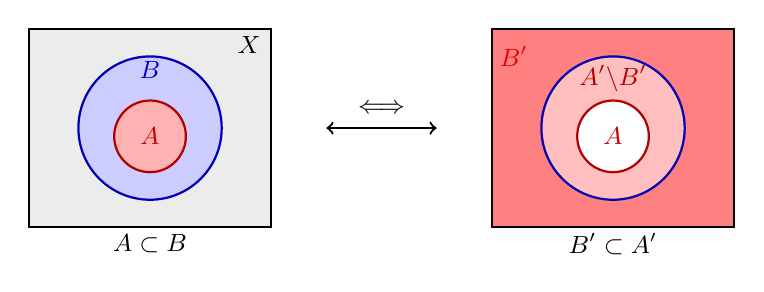
\begin{tikzpicture}[scale=0.7]

%--- LEFT DIAGRAM: A subset B ---
\begin{scope}[xshift=-4.2cm]
  \fill[gray!15] (-2.2,-1.8) rectangle (2.2,1.8);
  \draw[thick] (-2.2,-1.8) rectangle (2.2,1.8);
  \node[font=\small] at (1.8, 1.5) {$X$};
  
  % B large
  \fill[blue!20] (0,0) circle (1.3cm);
  \draw[thick, blue!70!black] (0,0) circle (1.3cm);
  \node[blue!80!black, font=\small] at (0, 1.05) {$B$};
  
  % A small inside B
  \fill[red!30] (0,-0.15) circle (0.65cm);
  \draw[thick, red!70!black] (0,-0.15) circle (0.65cm);
  \node[red!80!black, font=\small] at (0,-0.15) {$A$};
  
  \node[font=\small] at (0,-2.1) {$A \subset B$};
\end{scope}

%--- DOUBLE ARROW ---
\draw[thick, <->] (-1.0,0) -- (1.0,0);
\node[font=\small] at (0, 0.35) {$\iff$};

%--- RIGHT DIAGRAM: B' subset A' ---
\begin{scope}[xshift=4.2cm]

  % A' = everything outside A = shade whole universe red first
  \fill[red!25] (-2.2,-1.8) rectangle (2.2,1.8);

  % Inside A = white (not part of A')
  \fill[white] (0,-0.15) circle (0.65cm);

  % B' = everything outside B
  % Outside B but inside A = blue ring (part of A' since outside B means outside A too)
  % Wait — outside B includes the ring between A and B AND outside A
  % Ring between A and B is INSIDE A, so NOT in A'
  % So B' has two parts: ring inside A (not in A') and outside A (in A')
  % For B' subset A' we need the ring part to be empty
  % Which means A = B, but that contradicts A strict subset B...

  % UNLESS we allow A = B, in which case B' = A' exactly

  % The theorem says A subset B (not strict), so if A = B then B' = A' trivially
  % If A strict subset B, then ring between A and B exists
  % and that ring is in B' (outside B? NO — ring is INSIDE B, outside A)
  % Ring between A and B: inside B, outside A
  % So ring is in B (not B') and in A' (not A)
  % B' = outside B = outside the large circle = subset of outside A = subset of A'
  % YES this works — B' is only the region OUTSIDE the large B circle
  % which is entirely within A' (outside the small A circle)

  % So correct shading:
  % B' region = outside large circle = red (already done via A' shading above)
  % But B' is SUBSET of A', so B' region needs different shade

  % Redo:
  % Full universe gray
  \fill[gray!15] (-2.2,-1.8) rectangle (2.2,1.8);
  \draw[thick] (-2.2,-1.8) rectangle (2.2,1.8);
  \node[font=\small] at (1.8, 1.5) {$X$};

  % A' = outside small circle = red
  \fill[red!25] (-2.2,-1.8) rectangle (2.2,1.8);
  \fill[white] (0,-0.15) circle (0.65cm); % inside A = white

  % B' = outside large circle = darker red (subset of A')
  % Can't easily shade only outside large circle without clipping
  % Use scope + clip trick:
  \begin{scope}
    \clip (-2.2,-1.8) rectangle (2.2,1.8);
    % Shade everything, then remove inside B
    \fill[red!50] (-2.2,-1.8) rectangle (2.2,1.8);
    \fill[red!25] (0,0) circle (1.3cm); % inside B back to lighter red
    \fill[white] (0,-0.15) circle (0.65cm); % inside A white
  \end{scope}

  % Draw outlines
  \draw[thick, blue!70!black] (0,0) circle (1.3cm);
  \draw[thick, red!70!black] (0,-0.15) circle (0.65cm);
  \draw[thick] (-2.2,-1.8) rectangle (2.2,1.8);

  % Labels
  \node[red!80!black, font=\small] at (0,-0.15) {$A$};
  \node[red!70!black, font=\small] at (0, 0.9) {$A'{\setminus}B'$};
  \node[red!90!black, font=\small] at (-1.8, 1.3) {$B'$};
  \node[font=\small] at (0,-2.1) {$B' \subset A'$};

\end{scope}

\end{tikzpicture}
\end{center}

\section{Problems}

\begin{problem}
Prove by contradiction that $\sqrt{p}$ is irrational for any prime $p$.
\end{problem}

\begin{problem}
Prove that there is no integer solution to 
\[
n^4 - 4m = 2
\]
\hints{H49, H66}
\end{problem}

\begin{problem}
Let $a, b$ be integers. Prove that if $ab$ is odd, then both $a$ and $b$ are odd. \hints{H60, H77}
\end{problem}

\begin{problem}
Prove that for integers $a$ and $b$, if $a + b$ is even then $a$ and $b$ have the same parity (both even or both odd). Use proof by contrapositive.
\end{problem}

\begin{problem}
Prove that $\log_2 3$ is irrational. \hints{H65, H32, H10}
\end{problem}

\begin{problem}
Find, with proof, all integer solutions $(x, y) \in \mathbb{Z}^2$ to the equation
\[
x^2 + y^2 = 2027
\]
hints{H41, H44}
\end{problem}

\begin{problem}
Let $a, b, c$ be the side lengths of a triangle inscribed in a circle of radius $R$. Prove, using the inscribed angle theorem, that if the triangle is a right triangle then the hypotenuse must equal $2R$. Then prove the converse: if the hypotenuse equals $2R$, the triangle must be right-angled.

\hints{H50, H21} \hfill $\star$
\end{problem}

\begin{problem}
Prove that there are infinitely many primes of the form $4k - 1$. 

\hints{H47, H54, H67, H6, H12}\hfill $\star$
\end{problem}

\begin{problem}
Are there integers $a$ and $b$ such that $a^5b + 3$ and $ab^5 + 3$ are both perfect cubes of integers? Prove your answer. 

\hints{H17, H20, H86, H55, H8, H53, H24}\hfill \textit{2013 USAJMO \#1} $\star$
\end{problem}